\section{Laplace-Experimente} \label{section-laplace-ereignisse}
Bisher sind wir nicht in der Lage, die Wahrscheinlichkeit eines Ereignisses
zu berechnen, wir können nur mit Hilfe der Axiome aus bereits bekannten
Wahrscheinlichkeiten neue Wahrscheinlichkeiten berechnen.
Für die Berechnung der Wahrscheinlichkeiten ist zusätzliche
Information nötig.

Bei Experimenten mit endlich vielen Ausgängen ist es manchmal gerechtfertigt
anzunehmen, dass alle Versuchsausgänge gleich häufig und damit gleich
wahrscheinlich sind.
Von einem guten Würfel erwarten wir, dass er alle Seiten gleich häufig
zeigt, eine symmetrische Münze sollte Kopf und Zahl etwa gleich häufig
zeigen.
Unter dieser Annahme können wir die Wahrscheinlichkeit berechnen:

\begin{definition}
Ein Experiment mit $n=|\Omega|$ Ausgängen heisst ein {\em Laplace-Experiment},
wenn jeder Versuchsausgang gleich wahrscheinlich mit Wahrscheinlichkeit
\[
P(\{\omega\})=\frac1n,\qquad\omega\in\Omega
\]
ist.
\end{definition}

Da Laplace-Experimente nur endliche viele Ausgänge haben, kann man aus
den Axiomen auch jede andere Wahrscheinlichkeit berechnen:

\begin{satz}
Bei einem Laplace-Experiment tritt das Ereignis $A\subset\Omega$ mit
Wahrscheinlichkeit
\[
P(A)=\frac{|A|}{|\Omega|}
\]
ein.
\end{satz}
Damit ist die Berechnung der Wahrscheinlichkeit auf das Zählen der 
Versuchsausgänge in $A$ reduziert, also auf eine Kombinatorik-Aufgabe.

\subsection{Münze werfen}
\index{Munze@{Münze, faire}}
Wirft man eine Münze, kann sie nur auf einer von zwei Seiten landen,
die Elementarereignisse sind also $\Omega = \{\text{Kopf}, \text{Zahl}\}$.
Die mathematisch idealisierte Münze ist so dünn, dass sie nicht auf
der Kante stehen kann.
Nach allgemeiner Erfahrung funktioniert für
solche Münzen der Ansatz von Laplace, d.~h.~$P(\text{Kopf}) = \frac12$
und $P(\text{Zahl})=\frac12$.

Selbstverständlich gibt es auch Münzen, für die die Laplace-Annahme
nicht funktioniert, gebogene Münzen fallen zum Beispiel bevorzugt auf die
nach aussen gewölbte Fläche.

\subsection{Würfeln}
\index{Wurfel@{Würfel, fairer}}
Würfel haben sechs Seiten, die gemäss der Annahme eines Laplace-Experiments
mit gleicher
Wahrscheinlichkeit oben liegen werden, die Wahrscheinlichkeit jedes
Resultates ist also gleich $P(i) = \frac16, i\in\{1,2,3,4,5,6\}$.
Wird eine Seite des Würfels beschwert, fällt er bevorzugt auf diese
Seite, und die Wahrscheinlichkeiten sind nicht mehr gleich.

\begin{figure}
\begin{center}
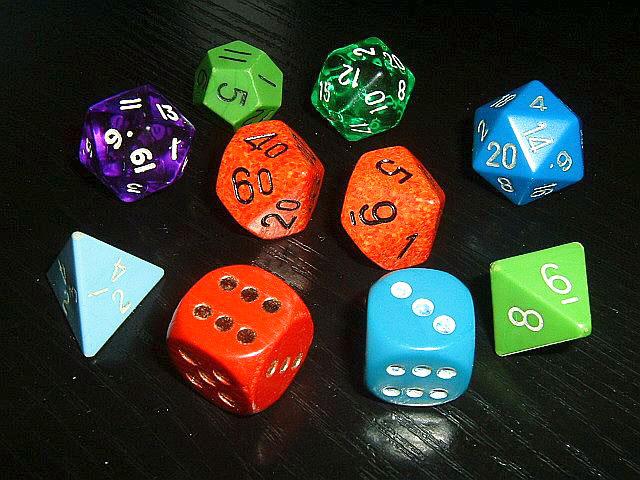
\includegraphics[width=0.8\hsize]{graphics/Wuerfel5}
\end{center}
\caption{Verschiedene Spielwürfel\label{bild-spielwuerfel}}
\end{figure}
Man kann auch aus anderen geometrischen Körpern ``Würfel'' bauen, die
eine grössere Zahl von Ausgängen ermöglichen.
Ein Dodekaeder hat
zwölf Seiten, ein Ikosaeder sogar deren 20, aber auch andere Formen
sind realisierbar, siehe Abbildung~\ref{bild-spielwuerfel}.
Der Einfachheit
halber gehen wir im Folgenden immer von sechsseitigen Würfeln aus.

Das Werfen eines solchen Würfels erzeugt die folgenden Elementarereignisse
oder Versuchsergebnisse:
\[
\Omega=\{1,2,3,4,5,6\}.
\]
Nach dem Laplace'schen Ansatz wird jedem Elementarereignis die
Wahrscheinlichkeit $\frac16$ zugeschrieben.
Damit lassen sich
Wahrscheinlichkeiten berechnen:
\begin{align*}
P(\text{``gerade Zahl''})=P(\{2,4,6\})&=\frac36=0.5\\
P(\text{``durch 3 teilbar''})=P(\{3,6\})&=\frac26=0.333\\
P(< 7)=P(\Omega)&=\frac66=1
\end{align*}

\subsection{Zwei Würfel}
In verschiedenen Spielen wird mit zwei Würfeln gespielt, wobei nur
deren Augensumme interessiert.
Die Ereignisalgebra dazu wurde bereits
früher vorgestellt, die Elementarereignisse sind Paare $(i,j)$ aus
den Augenzahlen der beiden Würfel.
Die Menge der Elementarereignisse
ist also
% hier brauchen wir wirklich ein eqnarray, wegen dem Spacing
\begin{eqnarray*}
\Omega=&\{&\\
&&(1,1),(1,2),(1,3),(1,4),(1,5),(1,6),\\
&&(2,1),(2,2),(2,3),(2,4),(2,5),(2,6),\\
&&(3,1),(3,2),(3,3),(3,4),(3,5),(3,6),\\
&&(4,1),(4,2),(4,3),(4,4),(4,5),(4,6),\\
&&(5,1),(5,2),(5,3),(5,4),(5,5),(5,6),\\
&&(6,1),(6,2),(6,3),(6,4),(6,5),(6,6),\\
&\},&
\end{eqnarray*}
und $|\Omega|=36$.
Wenn nur die Augensumme interessiert, dann will
man offensichtlich die Ereignisse
\begin{align*}
A_2&=\{\Sigma=2\}=\{(1,1)\}\\
A_3&=\{\Sigma=3\}=\{(1,2),(2,1)\}\\
A_4&=\{\Sigma=4\}=\{(1,3),(2,2),(3,1)\}\\
&\vdots\\
A_{12}&=\{\Sigma=12\}=\{(6,6)\}
\end{align*}
untersuchen.
Diese Ereignisse sind einfach auszuzählen, und damit kann man auch
die Wahrscheinlichkeiten bestimmen:
\begin{align*}
P(A_2)=P(A_{12})&=\frac{1}{36},\\
P(A_3)=P(A_{11})&=\frac{2}{36},\\
P(A_4)=P(A_{11})&=\frac{3}{36},\\
P(A_5)=P(A_9)&=\frac{4}{36},\\
P(A_6)=P(A_8)&=\frac{5}{36},\\
P(A_7)&=\frac{6}{36}.
\end{align*}

\subsection{Geburtstagsproblem}
Wie gross ist die Wahrscheinlichkeit, dass unter $n$ Personen zwei
am gleichen Tag Geburtstag haben? Hierbei nimmt man an, dass
jeder Tag im Jahr etwa gleich häufig als Geburtstag
vorkommt\footnote{Dies ist
jedoch nicht ganz richtig, wie Gebärabteilungen in Spitälern
bestätigen können.
Auch haben grössere Stromausfälle häufig
einen Geburtenzuwachs ungefähr neun Monate später zur Folge.}.
Ein Elementarereignis muss also jeder der $n$ Personen ein
Geburtsdatum aus den $366$ möglichen zuweisen.
Dies kann man so
formulieren:
\[
\omega=(d_1, d_2, d_3,\dots,d_n)
\]
Dabei ist $d_1$ das Geburtsdatum der ersten Person, $d_2$ das
Geburtsdatum der zweiten Person, etc.
Der Einfachheit halber kann
man für die $d_i$ einfach Zahlen zwischen 1 und 366 nehmen.

$\Omega$ besteht also aus allen möglichen Auswahlen von Geburtstagen
für die $n$ Personen:
% hier brauchen wir wirklich ein eqnarray, wegen dem Spacing
\begin{eqnarray*}
\Omega=&\{&\\
&&(1,1,1,\dots,1),\\
&&(2,1,1,\dots,1),\\
&&(3,1,1,\dots,1),\\
&&\dots\\
&&(365,1,1,\dots,1),\\
&&(366,1,1,\dots,1),\\
&&(1,2,1,\dots,1),\\
&&(2,2,1,\dots,1),\\
&&\dots\\
&&(366,366,366,\dots,366)\\
&\}&
\end{eqnarray*}
Man kann ablesen, dass $|\Omega|=366^n$ ist.

Gefragt ist nun das Ereignis
``zwei Personen haben am gleichen Tag Geburtstag''.
Selbstverständlich dürfen dabei auch alle am gleichen Tag
Geburtstag haben, oder es darf zwei Paare geben, die jeweils
übereinstimmende Geburtstage haben.
Es darf einfach nicht
sein, dass alle Geburtstage verschieden sind.
Also ist eigentlich
gemeint:
\begin{align*}
A&=\{\text{``zwei haben am gleichen Tag Geburstag''}\}\\
&=\{\text{``nicht alle Geburtstage sind verschieden''}\}\\
&=\overline{\{\text{``alle Geburstage sind verschieden''}\}}.
\end{align*}
In dieser letzten Form ist die Wahrscheinlichkeit einfacher zu
berechnen.
Es gilt ja:
\begin{align*}
P(A)&=P(\{\text{``zwei haben am gleichen Tag Geburstag''}\})\\
&=1-P(\{\text{``alle Geburstage sind verschieden''}\}).
\end{align*}
Die Anzahl der Geburtstagsverteilungen, bei denen alle Geburtstage
verschieden sind, ist einfach zu ermitteln: Für die erste Person
kann man $366$ Geburtstage auswählen, für die zweite $365$, die
dritte $364$ etc.
Insgesamt hat man
\[
366\cdot365\cdot364\dotsm(366-n+1)
\]
Möglichkeiten.
Also ist die Wahrscheinlichkeit, dass unter $n$
Personen zwei am gleichen Tag Geburtstag haben:
\[
P(A)
=
1-\frac{366\cdot365\cdot364\dotsm(366-n+1)}{366^n}
=
1-\frac{366}{366}\cdot
\frac{365}{366}\cdot
\frac{364}{366}
\dotsm
\frac{366-n+1}{366}
.
\]
Man kann diese Wahrscheinlichkeiten mit einem kleinen Programm
ausrechnen, und findet die Resultate in
Tabelle~\ref{geburtstagswahrscheinlichkeit}.
\begin{table}
\begin{center}
\begin{tabular}{|c|c|c|c|c|c|c|c|}
\hline
$n$&$P$&$n$&$P$&$n$&$P$&$n$&$P$\\
\hline
1&0.0000
&11&0.1408
&21&0.4428
&31&0.7295\\
2&0.0027
&12&0.1666
&22&0.4748
&32&0.7524\\
3&0.0082
&13&0.1939
&23&0.5063
&33&0.7740\\
4&0.0163
&14&0.2226
&24&0.5373
&34&0.7944\\
5&0.0271
&15&0.2523
&25&0.5677
&35&0.8135\\
6&0.0404
&16&0.2829
&26&0.5972
&36&0.8313\\
7&0.0561
&17&0.3143
&27&0.6258
&37&0.8479\\
8&0.0741
&18&0.3461
&28&0.6534
&38&0.8633\\
9&0.0944
&19&0.3783
&29&0.6799
&39&0.8775\\
10&0.1166
&20&0.4106
&30&0.7053
&40&0.8905\\
\hline
\end{tabular}
\end{center}
\caption{Wahrscheinlichkeit dafür, dass unter $n$ Personen zwei
am gleichen Tag Geburtstag haben.\label{geburtstagswahrscheinlichkeit}}
\end{table}
Ab $n=23$ kann man also wetten, dass zwei Personen am gleichen Tag
Geburtstag haben.

